\begin{center}
\begin{minipage}[t]{.46\linewidth}\vspace{0pt}\centering
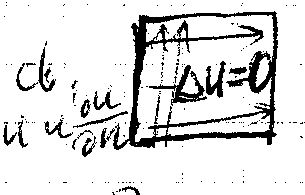
\includegraphics[width=\linewidth]{figures/gelfand-0153-p001406-boundary-original.png}\par\smallskip
{\footnotesize Оригинал рукописного рисунка: \texttt{GELFAND-P001406}}
\end{minipage}\hfill
\begin{minipage}[t]{.50\linewidth}\vspace{0pt}\centering
{\footnotesize Частичное воссоздание видимых штрихов}\par\smallskip
\resizebox{\linewidth}{!}{\begin{tikzpicture}[x=1.2cm,y=1.2cm]
\draw (0,0) rectangle (1.1,1);
\draw[->] (.05,.83)--(1.04,.83);\draw[->] (.03,.13)--(1.06,.19);
\draw[->] (.15,.1)--(.19,.95);\draw[->] (.29,.13)--(.36,.96);
\node at (.69,.55) {$\Delta u=0$};
\node[left] at (-.05,.6) {$[?]$};
\node[left] at (-.06,.05) {$u,\ \dfrac{\partial u}{\partial n}$};
\end{tikzpicture}
}
\end{minipage}
\end{center}
\noindent{\small\textit{Верхнее левое обозначение остаётся [?] после просмотра при 3×, 5× и 10×. Видимые u и нормальная производная набраны; граничное условие не дополнено.}}
